\section{Infinite Case}
\label{sec:Infinite Case}
\[
  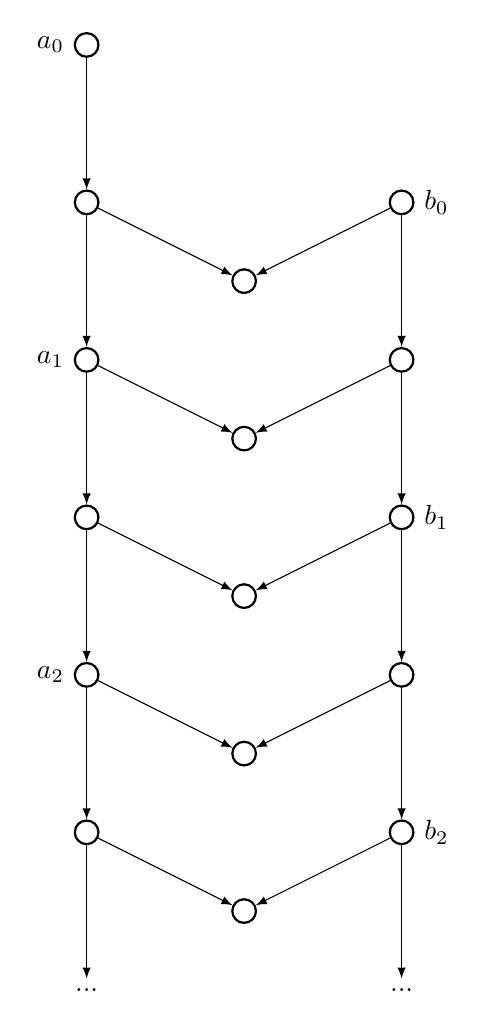
\begin{tikzpicture}
    [
    point/.style={thick,circle,draw,inner sep=0pt,minimum size=3mm},
    trimmed/.style={thick,draw=red},
    untrimmed/.style={thick,draw=black}
    ]
    \node (A0) at (0,12) [point,label=left:$a_0$] {};
    \node (A1) at (0,10) [point] {};
    \node (B1) at (4,10) [point,label=right:$b_0$] {};
    \node (C1) at (2,9) [point] {};
    \node (A2) at (0,8) [point,label=left:$a_1$] {};
    \node (B2) at (4,8) [point] {};
    \node (C2) at (2,7) [point] {};
    \node (A3) at (0,6) [point] {};
    \node (B3) at (4,6) [point,label=right:$b_1$] {};
    \node (C3) at (2,5) [point] {};
    \node (A4) at (0,4) [point,label=left:$a_2$] {};
    \node (B4) at (4,4) [point] {};
    \node (C4) at (2,3) [point] {};
    \node (A5) at (0,2) [point] {};
    \node (B5) at (4,2) [point,label=right:$b_2$] {};
    \node (C5) at (2,1) [point] {};
    \node (A6) at (0,0) [] {...};
    \node (B6) at (4,0) [] {...};
    \draw [-latex] (A0) to (A1);
    \draw [-latex] (A1) to (A2);
    \draw [-latex] (A1) to (C1);
    \draw [-latex] (B1) to (B2);
    \draw [-latex] (B1) to (C1);
    \draw [-latex] (A2) to (A3);
    \draw [-latex] (A2) to (C2);
    \draw [-latex] (B2) to (B3);
    \draw [-latex] (B2) to (C2);
    \draw [-latex] (A3) to (A4);
    \draw [-latex] (A3) to (C3);
    \draw [-latex] (B3) to (B4);
    \draw [-latex] (B3) to (C3);
    \draw [-latex] (A4) to (A5);
    \draw [-latex] (A4) to (C4);
    \draw [-latex] (B4) to (B5);
    \draw [-latex] (B4) to (C4);
    \draw [-latex] (A5) to (A6);
    \draw [-latex] (A5) to (C5);
    \draw [-latex] (B5) to (B6);
    \draw [-latex] (B5) to (C5);
  \end{tikzpicture}
\]
